\documentclass{article}

\author{Pedro Henrique Limeira da Cruz}
\title{Trabalho Final - ES101}

\usepackage[margin=0.8in]{geometry}
\usepackage{indentfirst}
\usepackage{fancyhdr}
\usepackage{tcolorbox}
\usepackage{graphicx}
\usepackage{amsmath}

% Create a new command to be used in the align environment in multiple line equations do only the last equation is numbered  
\newcommand{\n}{\nonumber \\ }
\makeatletter
\let\inserttitle\@title
\makeatother
% Set the style of the page 
\pagestyle{fancy}
\fancyhf{}
\rhead{Pedro Henrique L. da Cruz}
\lhead{\inserttitle}
\rfoot{Page \thepage}

\usepackage{hyperref}
\hypersetup{
    colorlinks=true,
    linkcolor=black,
    filecolor=magenta,
    urlcolor=cyan,
}

% Begin the Document 
\begin{document}

    \maketitle
    \thispagestyle{empty}

    % Add the image inside a figure in as the first page
    \begin{figure}[h]
        \begin{center}
            
\includegraphics[scale = 0.15]{/Users/pedrocruz/Documents/UNICAMP/ES101/ES101 - Robotic Arm/img/unicamp.png}
        \end{center}
    \end{figure}

    % Change to the Next page 
    \newpage
    \tableofcontents
    \newpage

    \section{Introdução e Definições}

        A matéria de resistência dos materiais que iremos estudar nada mais é do que a análise de mecânica estática, só que, dessa vez, para corpos que se deformam.
        Levando isso em consideração, teremos primeiro que revisar alguns conceitos importantes de estática, sendo eles, de modo geral:
        \begin{itemize}
            \item Modelos de Suporte e Vínculos
            \item Equilíbrio Estático : cargas simples, combinadas, carregamentos distribuídos, ...
        \end{itemize}

        \subsection{Modelos de Suporte e Vínculos}

            Como o nosso objetivo é modelar o sistema para aplicarmos os equacionamentos de estática (e mais para frente outros mais específicos de ResMat) precisamos, primeiro, ser capazes de
            identificar as forças que atuam sobre o corpo em análise. Por isso remos revisar as diferentes forças de reação que cada tipo de suporte gera em uma viga:

            \begin{table}[h]
                \begin{tabular}{|l|c|c|c|l|l|}\hline
                    \textbf{Nome} & \textbf{Exemplo} & \textbf{Representação} & \textbf{D.C.L} & \textbf{Descrição} & \textbf{Cometário} \\ \hline

                    Rolete & 

                        \begin{minipage}{.2\textwidth}
                            \centering
                            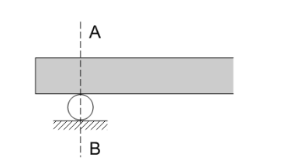
\includegraphics[width=\textwidth]{imgs/rolete_eg.png}
                        \end{minipage} &

                        \begin{minipage}{.2\columnwidth}
                            \centering
                            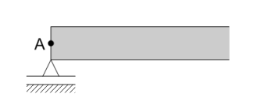
\includegraphics[width=\textwidth]{imgs/rolete_rep.png}
                        \end{minipage} &

                        \begin{minipage}{.2\columnwidth}
                            \centering
                            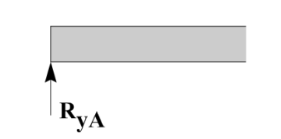
\includegraphics[width=.85\textwidth]{imgs/rolete_dcl.png}
                        \end{minipage} &

                        \begin{minipage}{.1\columnwidth}
                            \tiny
                            •Resistente a forças em \emph{somente uma linha de direção}

                                •Reação de apoio: 1 incógnita
                        \end{minipage}&

                        \begin{minipage}{.1\columnwidth}
                            \vspace{5px}
                            \tiny
                            Importante observar que a representação possui \textbf{DUAS} linhas horzontais abaixo do triângulo.
                            \vspace{5px}
                        \end{minipage} \\ \hline

                    Pino & 

                        \begin{minipage}{.2\textwidth}
                            \centering
                            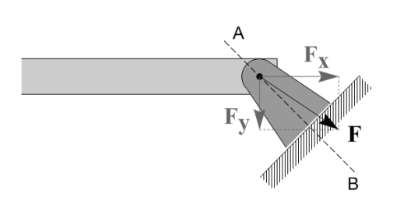
\includegraphics[width=\textwidth]{imgs/pino_eg.png}
                        \end{minipage} &

                        \begin{minipage}{.2\columnwidth}
                            \centering
                            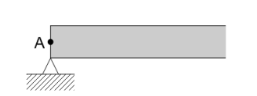
\includegraphics[width=\textwidth]{imgs/pino_rep.png}
                        \end{minipage} &

                        \begin{minipage}{.2\columnwidth}
                            \centering
                            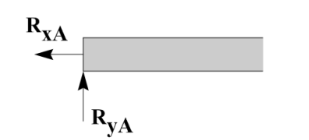
\includegraphics[width=\textwidth]{imgs/pino_dcl.png}
                        \end{minipage} &

                        \begin{minipage}{.1\columnwidth}
                            \tiny
                            •Resistente a forças em \emph{duas linhas de ação}

                            •Reação de apoio: 2 incógnitas
                        \end{minipage}&

                        \begin{minipage}{.1\columnwidth}
                            \vspace{5px}
                            \tiny
                            Importante observar que a representação possui somente \textbf{UMA} linha horzontai abaixo do triângulo.
                            \vspace{5px}
                        \end{minipage} \\ \hline


                        Engaste & 

                            \begin{minipage}{.2\textwidth}
                                \centering
                                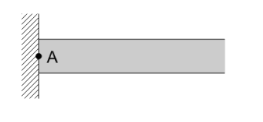
\includegraphics[width=\textwidth]{imgs/engaste_rep.png}
                            \end{minipage} &

                            \begin{minipage}{.2\columnwidth}
                                \centering
                                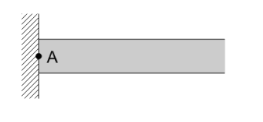
\includegraphics[width=\textwidth]{imgs/engaste_rep.png}
                            \end{minipage} &

                            \begin{minipage}{.2\columnwidth}
                                \centering
                                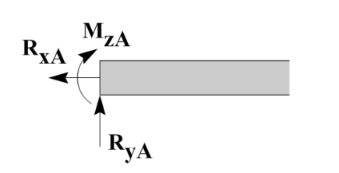
\includegraphics[width=\textwidth]{imgs/engaste_dcl.png}
                            \end{minipage} &

                            \begin{minipage}{.1\columnwidth}
                                \tiny
                                • Resiste a \textbf{Forças} e \textbf{Momentos}
                            \end{minipage}&

                            \begin{minipage}{.1\columnwidth}
                                \vspace{5px}
                                \tiny
                                Até o momento é o único vínculo que resiste a momento.
                                \vspace{5px}
                            \end{minipage} \\ \hline

                \end{tabular}
                \caption{Principais Suportes e Vínculos - 2D}
            \end{table}

        \subsection{Cargas Combinadas}

            Pela tabela acima temos os principais suportes e suas característica. Quando estamos analisando problemas complexos (com diversas forças), entretanto, os modelos acima podem
            \textbf{não serem suficientes para modelarmos todas forças e momentos presentes ao mesmo tempo}. Nesses casos, é encessário escolher o tipo certo de suporte e vínculo para a força que está sendo
            analisada no momento (e por conseguinte várias análises serão necessárias).

            Tenso isso em vista, é importante entender o processo de escolha de vínculos durante análise de uma força. Para tal, podemos nos perguntar:
            \begin{enumerate}
                \item \textbf{O apoio/vínculo impede algum movimento que será resultante da força sob análise?} Se a resposta for \emph{não}, podemos simplesmente desconsiderar o vinculo na nossa
                modelagem. Se a resposta for \emph{sim}, ele impede um movimento, podemos prosseguir para outras perguntas.
                \item \textbf{O apoio/vínculo impede que a peça "gire" como resultado da força?} Se a resposta for \emph{sim} isso significa que o suporte restringe tanto forças quanto
                \emph{momentos}. Como temos somente um vínculo (o engaste) que tem essa característica, podemos usa-lo durante nossa modelagem. Se a resposta for não, fiamos entre um rolete e um pino.
                \item \textbf{O apoio/vínculo impede a movimentação, que seria resultante da força, em mais de um eixo?} Se \emph{sim}, temos um pino. Caso contrário teremos um rolete.
            \end{enumerate}

        \subsection{Equilíbrio Estático}

            Como dito anteriormente, o ponto de partida de ResMat é a estática mecânica. Agora que já definimos os principais modelos de forças de reação, podemos descrever o equilíbrio estático
            (assim como foi feito durante o estudo de Estática).

            O principal conceito que rege o equilíbrio estático é que o sistema não possui aceleração, logo há a conservação tanto da quantidade de movimento linear quanto angular, resultando nas
            respectivas equações:

            $$\\$$

            \begin{minipage}{.5\linewidth}
                \begin{align*}
                    \sum \vec F = 0 \Rightarrow \begin{cases}
                        \sum F_x = 0 \\ 
                        \sum F_y = 0 \\ 
                        \sum F_z = 0
                    \end{cases} 
                \end{align*}
            \end{minipage}%
            \begin{minipage}{.5\textwidth}
                \begin{align*}
                    \sum \vec M = 0 \Rightarrow \begin{cases}
                        \sum M_x = 0 \\ 
                        \sum M_y = 0 \\
                        \sum M_z = 0
                    \end{cases}
                \end{align*}
            \end{minipage}


            $$\\$$

            Para problemas de sistemas planos, as equações se resumem à:

            $$\\$$

            \begin{minipage}{.5\textwidth}
                    \centering
                    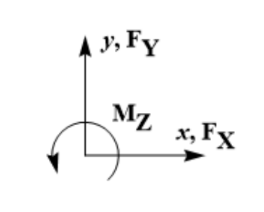
\includegraphics[width=.5\textwidth]{imgs/sis_plano.png}
            \end{minipage}%
            \begin{minipage}{.5\textwidth}
                \begin{align*}
                    \sum F_x = 0 \\ 
                    \sum F_y = 0 \\ 
                    \sum M_z = 0
                \end{align*}
            \end{minipage}

            A depender da topologia, no que tange equilíbrio estático, um sistema pode ser definido como:
            \begin{itemize}
                \item \textbf{Sistema Isostático}: As vinculações são suficientes para satisfazer o equilíbrio estático, número de incógnitas igual ao numero de equações.
                \item \textbf{Sistema Hiperestático}: As vinculações são em excesso para satisfazer o equilíbrio estático, número de incógnitas maior ao numero de equações.
                \item \textbf{Sistema Hipostático}: As vinculações não são suficientes para satisfazer o equilíbrio estático, número de incógnitas menor ao numero de equações.
            \end{itemize}


    
\end{document}